\chapter{Introduction}

Our Universe's origin has always been a mystery until such time, when humankind started looking for answers to the unanswered questions about the evolution of the cosmos. The search for solutions led to a field of study called cosmology. This field has drastically impacted our knowledge of the universe's evolution~\citep{book:909085}.

Humans initially believed that the Sun, the moon, and other planets orbited the Earth until Nicolaus Copernicus and other astronomers replaced the geocentric model with the heliocentric model~\citep{sep-copernicus, kanas}.  Celestial mechanics emerged as an area of study after Isaac Newton discovered that elliptical planet motion can be explained by gravitational force attraction~\citep{crowe2013theories,sep-copernicus}. In the modern study of the Universe, our understanding of gravity has been further refined by Albert Einstein's theory of general relativity, which presents the mathematical framework required to describe the evolution of the universe.
	
As a result of all these findings \attention{[you haven't discussed ``these findings'' yet---discuss the discovery of the expanding universe and the CMB first, before introducing the big bang model]}, Georges Lemaitre proposed the Big Bang theory, the contemporary model that provides a complete explanation of the Universe expansion~\citep{1926ApJ....64..321H}. The Big Bang theory was established from Hubble's law and subsequently by Arno Penzias and Robert Wilson in 1964 from discovering the cosmic microwave background (CMB)~\citep{1965ApJ...142..419P,2003RvMP...75..559P,1929PNAS...15..168H}. The Supernova Cosmology Project and the High-Z Supernovae Search Team in 1998 discovered the acceleration of the Universe using observations of type Ia supernovae~\citep{1998AJ....116.1009R, 1999ApJ...517..565P}. The accelerated expansion is described by dark energy, which accounts for approximately 74 percent of the Universe's energy density. Today, understanding the nature of dark energy is a major area of focus in astrophysics and particle physics~\citep{2008ARA&A..46..385F}. 
	
	\section{History of the Universe}
	
	\autoref{Fig:timeline} shows the cosmic history of the Universe. The Planck era, which lasted unil \SI{e-43}{s} after the big bang is unknown to physicists and requires a quantum theory of gravity. Following the Planck era, \SI{e-34}{s} after the big bang, the universe went through a period of rapid exponential expansion, known as Inflation~\citep{1981PhRvD..23..347G}.

	\begin{figure}
		\begin{center}
			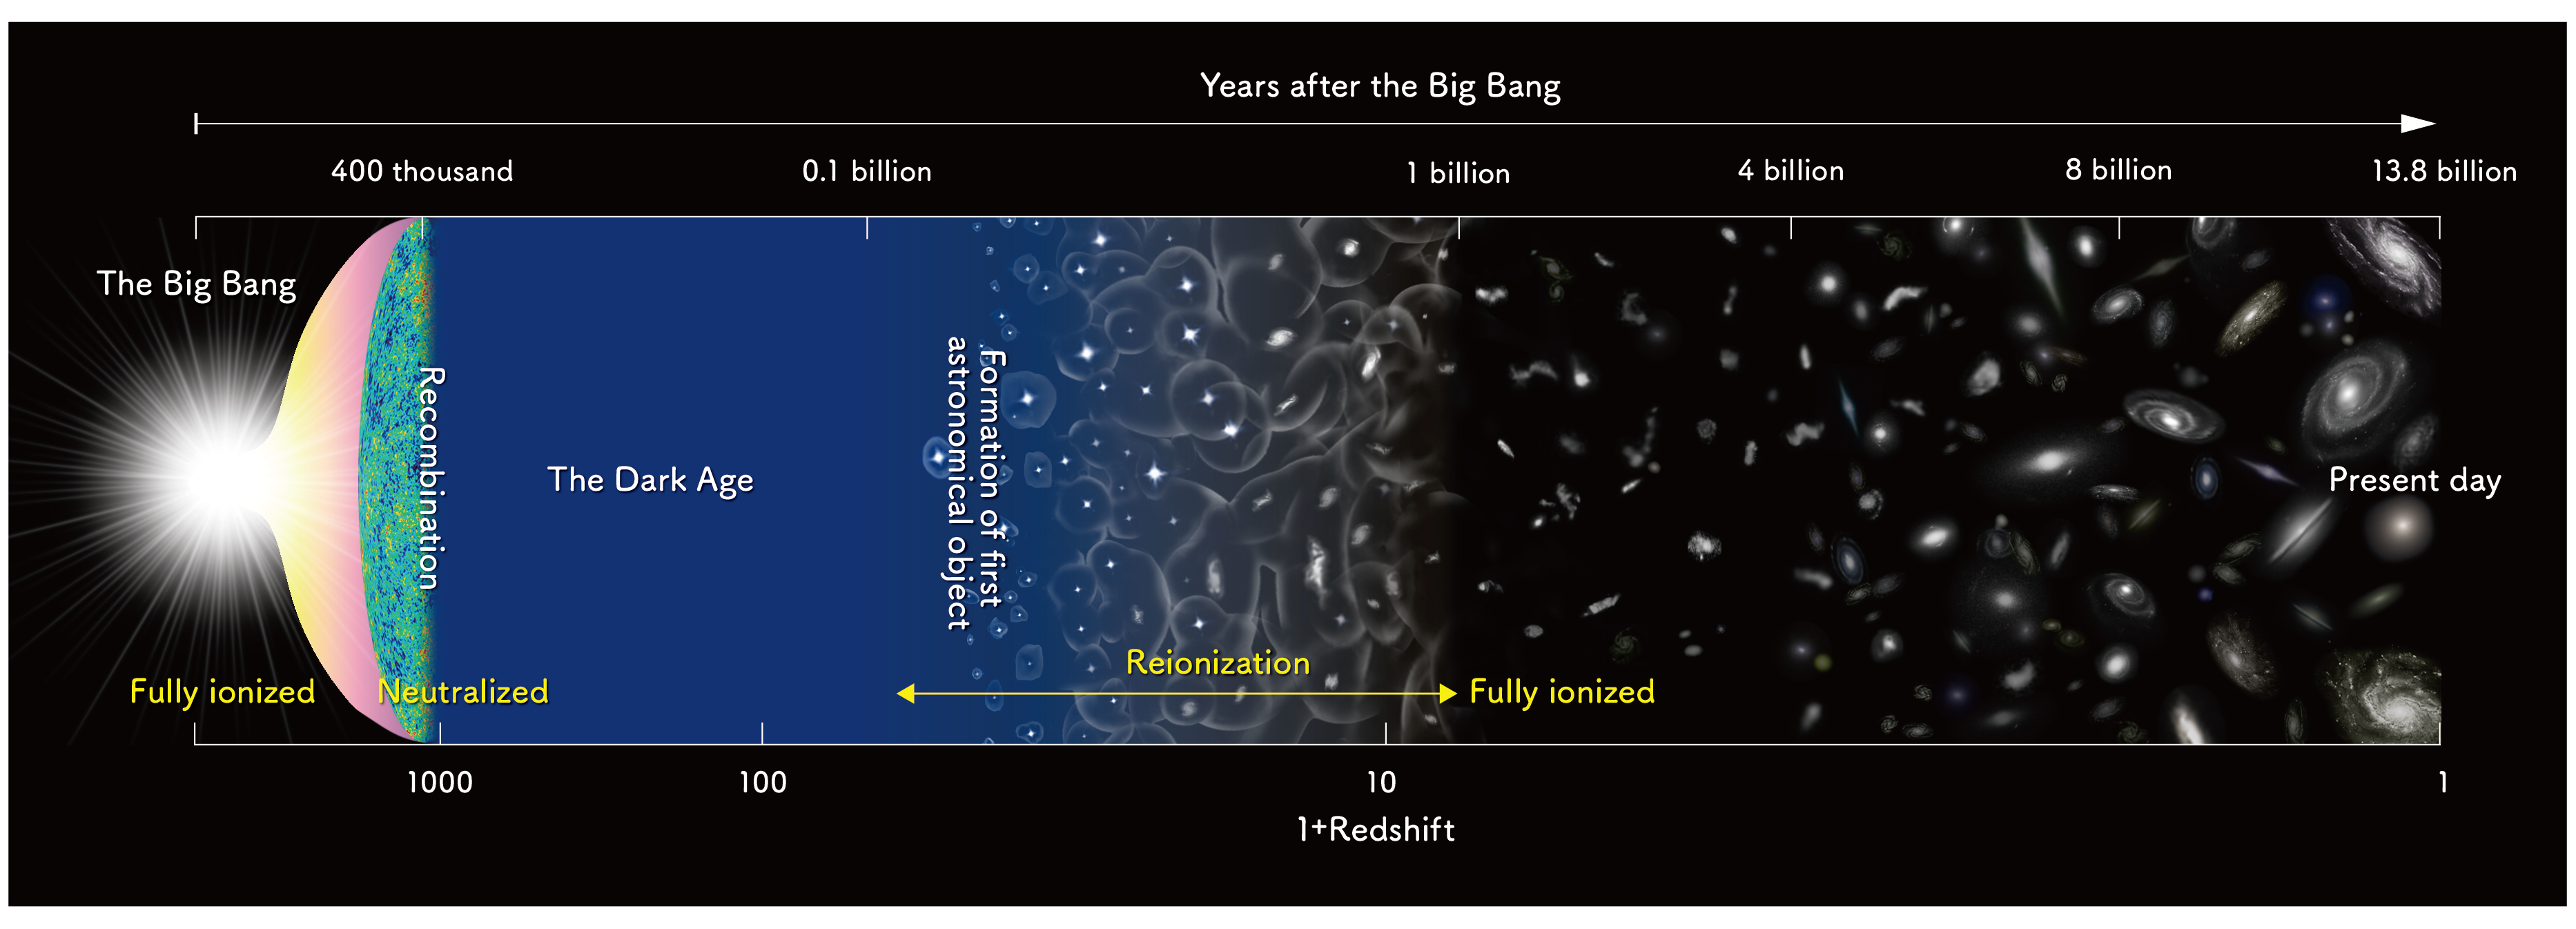
\includegraphics[width=\linewidth]{Figures/Reionizationtimeline.jpg}
			\caption{The cosmic history of the Universe from the Big Bang to its early years, through the dark ages to the epoch of reionization and the post-reionization epoch. Image credit:National Optical Astronomy Observatory}
			\label{Fig:timeline}
		\end{center}
	\end{figure}
        
	Recombination occurred when the universe cooled enough for neutral hydrogen (HI) to form, around a redshift of $z$ $\sim1100$. The redshift-wavelength relation is \attention{[include a brief phrase here describing what redshift physically means, i.e. that higher redshift means earlier times] given} by
	\begin{equation}
	\begin{split}
	1+z & = \frac{\lambda_{obs}}{\lambda_{emit}}= \frac{1}{a}
	\end{split}
	\end{equation}
	where $z$ is the redshift, $\lambda_{obs}$ is the wavelength of the observed signal, $\lambda_{emit}$ is the wavelength of the signal emitted, and $a$ is the Universe expansion scale factor. Prior to recombination, electrons were not bound to protons, and the Universe contained ionized plasma known as photon-baryon fluid. Decoupled photons then formed the CMB~\citep{1965ApJ...142..419P}.

	Subsequently, HI became the dominant baryonic component of the intergalactic medium (IGM) during the dark ages ($1100 \gtrsim z \gtrsim 30$). No measurements of the dark ages exist, and if hydrogen can be mapped in this era, valuable cosmological data can be produced~\citep{11, 2004PhRvL..92u1301L}.
	
	There were density fluctuations in the distribution of matter, and the overdense regions collapsed under the influence of gravity, ultimately creating the first stars. Thus, nuclear reaction resulted in Cosmic Dawn ($30\gtrsim z \gtrsim 10$). Energy from the first stars ultimately fully reionized the Universe. Galaxies, galaxy clusters and large-scale structures that exist in the present universe evolved after the first stars were born~\citep{2017arXiv170808521D, 2012AdSpR..49..433B}. 
	
	Throughout the cosmological epochs, what is known is minimal because it is challenging to observe them directly. The growth of \SI{21}{cm} cosmology has the capability to fill the gaps in our knowledge of the universe's history~\citep{2012RPPh...75h6901P}. A brief overview of the history of the Universe has been given, and the next section will cover 21 cm cosmology corresponding to the dark ages and cosmic dawn in more detail.
	           
	\section{Cosmology with Redshifted 21-cm Emission}
		
	Because hydrogen gas is the most abundant element in the universe, there is a concerted effort in the experimental community to develop telescopes for mapping neutral hydrogen via \SI{21}{cm} emission. This hydrogen line is an essential mechanism for probing the dark ages to the epoch of reionization (EoR)~\citep{2013PhRvD..87d3002L,2014ApJ...782...66P}. The generation of the hydrogen line (\SI{21}{cm} line or HI line) is due to the intrinsic spins of the electron and proton within the hydrogen atoms~\citep{book:832129}. The electron and proton spins can be oriented in either the opposing or the same direction respective to each other. When the spins are opposing or antiparallel, the hydrogen atom is in the lower energy state. When the spins are parallel, the hydrogen atom is in a higher energy state. When an electron transitions from one state to another photon is emitted only when the transition is from the higher to the lower state, the hydrogen atom discharges a photon with a \SI{21}{cm} wavelength, equivalent to \SI{1420}{MHz}. The hyperfine splitting of the two energy states is equivalent to \(\Delta E =  5.9 \times 10^{-6} \ eV\). \autoref{Fig:21cm} shows the spin-flip transition process~\citep{16, book:832129}.
	
	\begin{figure}
		\begin{center}
			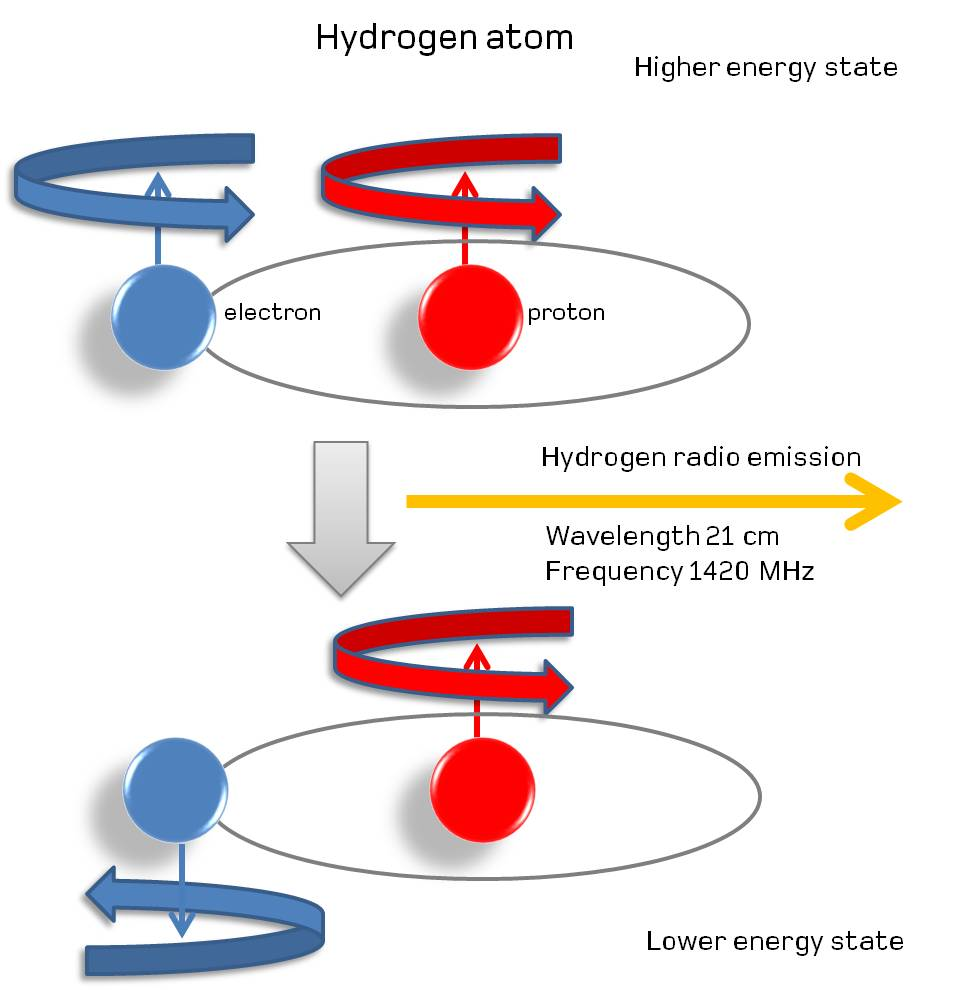
\includegraphics[width=0.5\linewidth]{Figures/Hydrogenemission1.jpeg}
			\caption{The formation of the \SI{21}{cm} wavelength line by the process of the spin flip transition where the hydrogen atom moves from one energy state to another. Image credit: {Square Kilometre Array}.}
			\label{Fig:21cm}
		\end{center}
	\end{figure}
	
	The populations of the low- and high-energy spin states, $n_0$ and $n_1$, define the spin temperature $T_s$:
	\begin{equation}
	\frac{n_0}{n_1} = \frac{g_1}{g_0}e^{(-E_10)/{k_B}{T_s}} = 3e^{{-T_*}{T_s}}.
	\end{equation}
	Here $\frac{g_1}{g_0}$ = 3 is the spin degeneracy of the triplet and singlet levels, and $T_{*}$ $\equiv$ $hc/k$ $\lambda_{21cm}$ = 0.068 K which is the equivalent temperature of the hyperfine splitting of the two energy levels~\citep{2012RPPh...75h6901P}.
	
	The brightness temperature $\delta$$T_b$ depends directly on $x_{HI}$, $z$, $T_S$, and $T_{CMB}$, but $T_S$ is heavily influenced by $T_K$ and the various coupling mechanisms. $x_{HI}$ is the fraction of neutral hydrogen, the hydrogen spin temperature ($T_S$) is the excitation temperature of the 21 cm line, kinetic gas temperature, $T_K$, characterizes the thermal motion of atoms in the gas~\citep{2015aska.confE...1K,2006PhR...433..181F}. The equation	
	\begin{equation}
	\delta{T_b}\propto {x_{HI}}(1+z)^{1/2}({T_s}-{T_{CMB}})/{T_s}
	\end{equation}
	relates $\delta$$T_b$ to important factors which are \(x_{HI}\), the fraction of neutral hydrogen, redshift ($z$) and two temperatures, the spin temperature ($T_s$) and the CMB temperature ($T_{CMB}$).
		
	Figure~\ref{Fig:epochs} describes the physical processes that are responsible for the frequency structures we see in the evolution of the sky-averaged 21 cm brightness temperature.
	
	\begin{figure}
		\begin{center}
			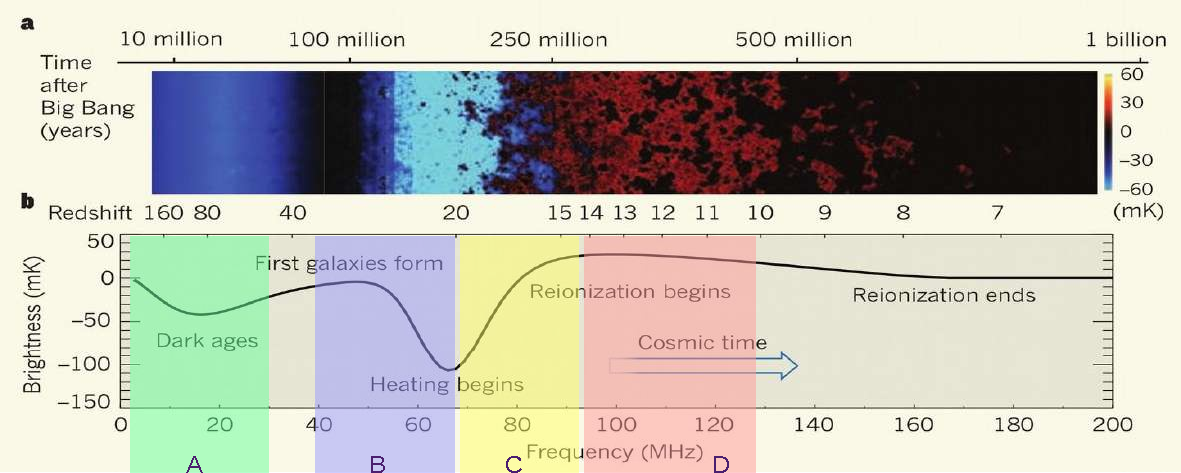
\includegraphics[width=\linewidth]{Figures/epo.pdf}\\
			\caption{Frequency structure of the globally averaged 21 cm signal: (a) shows the spatial and temporal evolution of the 21 cm brightness temperature and (b) shows the predicted time evolution of the globally averaged 21 cm brightness temperature ~\citep{2012RPPh...75h6901P}. There are different physical processes that govern the four highlighted (A to D) periods and the details are discussed in the main text.}			
			\label{Fig:epochs}
		\end{center}
	\end{figure}
	
	\subsection{Dark Ages}
	
	The cosmic dark ages lie between recombination and cosmic dawn, beginning $\sim380,000$ years after the big bang and ending a few tens of million years later ($1100 > z > 30$),~\citep{2014arXiv1412.2096J} during which there were no luminous sources. The cosmic dark ages possess distinctive features that have never been explored to date. 
	
	\textbf{Region A} in Figure~\ref{Fig:epochs} (green) highlights the dark ages period where the free electrons were no longer present. During this epoch, right after recombination, $T_K$=$T_\gamma$=$T_S$ where $T_\gamma$ is the temperature of the radiation background, typically set by the CMB so that $T_\gamma$ = $T_{CMB}$. During this period, matter that had separated from the CMB was cooled adiabatically as the Universe expanded, which led to $T_K$ decreasing below $T_\gamma$~\citep{2006PhR...433..181F}. $T_S$ is initially coupled to $T_K$ as the collision between hydrogen atoms is effective at early times, resulting in $\delta T_b$ decreasing. As the Universe expands and collisional coupling becomes ineffective, $T_S$ reverts to $T_\gamma$ because of CMB absorption, and $\delta T_b$ therefore eventually increases.
	
	At this juncture, the most dominating matter in the Universe was the dark matter and meager amounts of ordinary matter (neutral hydrogen and helium). After a few hundred million years, the dark and normal matter collapse together into halo-like structures through gravitational collapse, steadily cumulating physical matter and finally forming the first stars and galaxies, and that was the end of the cosmic dark ages~\citep{2003Sci...300.1904M}.
		
	\subsection{Cosmic Dawn}
	    
	    After the first stars' formation, their UV radiation couples to the HI line through the Wouthuysen-Field effect~\citep{2012RPPh...75h6901P}. Emission of Lyman Alpha photons by the first stars strongly couples $T_K$ and $T_S$ of the IGM; the described period is shown in \textbf{Region B} highlighted in purple. The coupling of $T_S$ to $T_K$ leads to a drastic absorption feature in $\delta T_b$. The absorption feature can be used to probe the formation processes of the first stars, with the potential of differentiating between Pop II and Pop III stars. \textbf{Region C} highlighted in yellow shows a period where the X-rays are emitted by hot accretion disks around the first stellar remnants (e.g., black holes) that effectively heat the cold HI gas. The heating of the neutral gas and continued coupling between $T_S$ and $T_K$ raised the overall spin-temperature to higher than the CMB temperature. Consequently, the 21-cm line became visible in emission at $z\sim15$. During radiation and heating, these first sources (possibly including mini-quasars) also ionized the gas around them, and a period of reionization started that is thought to have lasted until $z\sim5~to\sim 6$~\citep{2015aska.confE...1K}). The detailed $\delta T_b$ features are sensitive to the black hole properties and the progenitor's metallicity, offering further insight into first-star formation.~\citep{11}. \textbf{Region D} highlited in red describes that when reionization begins, the neutral hydrogen supply is depleted ($x_{HI}$ decreases to zero), so $\delta T_b$ eventually also flatlines to zero because there is no more 21 cm signal left. 
	    
	    \section{Hydrogen Line Observational Challenges}
	    
	    Redshifted 21-cm radiation can penetrate dust and the Earth's atmosphere and is therefore an ideal tool for probing the history of the Universe at any epoch of interest. However, ground-based telescopes and experiments are faced with several challenges when it comes to using the redshifted \SI{21}{cm} line emission to observe the dark ages, cosmic dawn, and the epoch of reionization. The primary challenges are human-made radio frequency interference (RFI), astrophysical foregrounds, ionospheric interference, and instrumental systematics which is non-transparent below 10 MHz. 
	    
	    \subsection*{Brightness of Foreground Emission}
	    
	    Foreground emission arises from both Galactic and extragalactic sources. The brightness temperatures of the foreground emission are 4-5 orders of magnitude brighter than the cosmological \SI{21}{cm} signal, which is $\sim$ 0.14 mK at $z\sim0.8$ \attention{[the focus of your thesis is the dark ages + cosmic dawn, so you should quote a temperature at a redshift that's more relevant to your work than 0.8]}. Galactic synchrotron emission is the primary foreground at low frequency and originates from the cosmic ray electrons' movement in the Galactic magnetic field. Free electrons scattering off ions without being captured produces the Galactic free-free emission. The extragalactic foregrounds are predominantly radio-loud galaxies and quasars~\citep{2018RAA....18..114H, 2008MNRAS.389.1319J}.
	    
	    \subsection*{Instrumental Systematics}\label{s:chall}

            \attention{[This section needs a rewrite.  Your text primarily addresses effects that are relevant for experiments that are aiming to detect 21-cm power spectra and fluctuations.  You should focus on the fact that global signal experiments measure total power and are therefore dominated entirely by systematics.  (For global experiments, there are no Fourier modes to speak of; we measure only the monopole.)  This would be a good section to include the order-of-magnitude estimate for the amount of integration time needed to detect the cosmic dawn feature assuming statistical noise alone---the answer is like a day of data.  If you haven't gone through this exercise with the radiometer equation, take a look at the description in Erika's senior thesis writeup at \url{http://www.physics.mcgill.ca/~chiang/theses/hornecker.pdf}.]}
            
	    There needs to be a precise calibration of instrumental systematics to remove instrument effects from the data.
	    
	    Instrumental systematics further complicate this effort, causing foreground signal to contaminate Fourier modes in the data that would otherwise only be noise limited. Instrumental systematics have limited many of the current upper limits on the 21 cm power spectrum. Therefore, precise modeling and separation of instrumental systematics will likely be necessary for second-generation 21 cm observations to make sturdy observations of the 21 cm cosmological signal. Instrumental systematics includes calibration errors, ionospheric faraday rotation, primary beam ellipticity, analog signal chain imperfections (such as impedance mismatches), internal instrument couplings, such as signal chain reflections, and antenna cross-coupling (i.e., crosstalk)~\citep{2020ApJ...888...70K}.
	    	    
	    \subsection*{RFI}
	    
	    Besides astrophysical challenges, human-made RFI saturates the frequency bands, increasing the need for isolated remote deployment sites. RFI can be orders of magnitude brighter than Galactic and extragalactic foregrounds. Unfortunately, RFI introduces a reduction in sensitivity in two separate but distinct ways: direct contamination by having similar spectral characteristics and overpowering the 21cm signal. The other is the introduction of a complex sampling function due to missing data. \attention{[Again, the latter is relevant for power spectrum/fluctuation experiments.  In this section, you should emphasize the fact that the cosmic dawn signal coincides with the FM band, and FM contamination is especially pervasive.]} This produces correlations between modes when computing the Fourier transform along the frequency axis. Therefore,  identifying RFI while not falsely identifying non-RFI as RFI is crucial, further complicating our sampling function over frequency~\citep{2019MNRAS.488.2605K}. \attention{[Same comment as before: you need to focus on RFI effects for global signal experiments, not power spectrum/fluctuation experiments.  If you need help getting some background information, I suggest asking people like Fernando, Raul, and Matheus if they'd be willing to schedule a chat with you.]}
	    
	    \subsection*{Ionospheric Contamination}
	    
	    The Earth's ionosphere also introduces significant fluctuations, which becomes increasingly refractive and turbulent below 100 MHz and becomes practically opaque below 10 MHz. In order to minimize RFI and ionospheric contamination, there have been proposals to observe long wavelengths from space-based telescopes further away from the ionosphere of our planet. These space-based telescopes do not exist yet, and there are several ground-based experimental efforts to understand how well we can make measurements from Earth~\citep{2019arXiv190710853C, 2019arXiv190804296K}. \attention{Also, as a prelude to chapter~2, mention that near-polar latitudes at night have lower plasma cutoff frequencies, and that the cutoff is reduced during solar minima.}
	    
	    \section{Previous Cosmic Dawn and Low-frequency Experiments}
	    
	    The \SI{21}{cm} wavelength of hydrogen gas is being observed by several experiments that are modeled for Hydrogen mapping in our Universe. Despite the challenges that are encountered in 21 cm cosmology, many experiments are nevertheless underway. This section highlights experiments aimed at frequencies corresponding to the dark ages ($1100 \lesssim z \lesssim 30$) and cosmic dawn ($30 \lesssim z \lesssim 10$).
	    
	    \subsection{Global Signal Experiments for Cosmic Dawn}

\attention{[Open with a general sentence describing the ``common denominator'' architecture for global signal experiments: a single antenna with a large solid angle observing total power, located in a remote, RFI-quiet place.]}
            
	    The Experiment to Detect the Global EoR Signature (EDGES) is located at Murchison Radio-astronomy Observatory (MRO) in Western Australia. The goal of the project is radio detection of characteristic hydrogen signatures from cosmic dawn and the epoch of reionization. EDGES consists of a high-band instrument operating over the 90-200 MHz (14 $>$ z $>$ 6) range, a mid-band instrument operating over 60–160 MHz, and a low-band instrument that is sensitive to the 50-100 MHz (27 $>$ z $>$ 13) range~\cite{2017ApJ...835...49M}. \attention{[WHOA, pull the car over: this paragraph needs to be at least 2--3 times longer to include a discussion of the detection (which you should also make sure to cite)!]}

\attention{[In this section, I would recommend describing EDGES and their detection in some detail, and then summarize all of the other experiments in a table rather than in paragraphs.  For your table, I'll suggest including the experiment name, location, observing frequencies, a brief phrase describing the instrumental approach (e.g. N dual-polarization dipoles, monopole antenna, etc.), and a citation.  I'll also suggest restricting your list to active and upcoming experiments: EDGES, SARAS2(3), LEDA, CTP, MIST, REACH, PRIZM...in alphabetical order, to be impartial.  Bighorns is no longer active and therefore shouldn't be included.]}
            
	    The Large aperture Experiment to Detect the Dark Ages (LEDA) experiment operates as part of the Long Wavelength Array at the Owens Valley Radio Observatory (LWA-OVRO). The LWA-OVRO array consists of 251 dual-polarized dipole antennas in a \SI{100}{\meter} radius circle and five outrigger antennas were fitted with LEDA instrumentation. LEDA operates in the frequency range 10–88 MHz. The instrumentation of LEDA facilitates \textit{in situ} characterization of the foreground, monitoring the ionosphere, and measuring antenna gain patterns during observations~\citep{2012JAI.....150004T, 2018MNRAS.478.4193P}.
	    	    
	    \subsection{Imaging below 30 MHz}
	    
	    {\bf{Long Wavelength Astronomy Background}}
	    
	    The father of radio astronomy, Karl G. Jansky, played a massive role in the inauguration of radio astronomy dating back to 1931. At that time, he was an employee at the Bell Telephone Laboratories as a radio engineer. Jansky was allocated to study and solve the problem that hindered the radio communication systems. Using highly directive antenna arrays shown in \autoref{Fig:Jansky}, he discovered that the static caused the radio frequency noise that hindered the communication systems from thunderstorms~\citep{book:BasicsofRA, book:RA}.
	    
	    \begin{figure}
	    	\begin{center}
	    		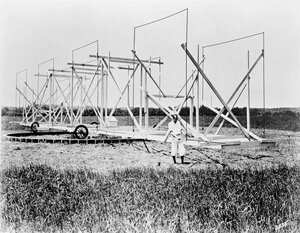
\includegraphics[width=0.7\linewidth]{Figures/jansky1.jpg}
	    		\caption{Jansky's highly directive antenna arrays which he used to discover the cause of RFI that hindered the communication systems at Bell Telephone Laboratories~\citep{book:BasicsofRA}}.
	    		\label{Fig:Jansky}
	    	\end{center}
	    \end{figure}
	    
	    The antenna that he constructed operated at an approximated frequency of \SI{20}{MHz}, corresponding to an approximate long wavelength of \SI{15}{m}. He further found radio radiation from the Galactic Center at the operating frequency. Out of interest in Jansky's instigating discoveries, Grote Reber designed a radio telescope that operated at a range of approximately \SI{10}{MHz} to \SI{160}{MHz} (\SI{30}{m}-\SI{2}{m} wavelength) in 1937. He discovered that the authoritative source at longer wavelengths was the Milky Way area. Furthermore, he realized that the radio telescope acts like a bolometer or a device to measure the heat. The antenna's radiation resistance measures an equivalent temperature of a distant part of space to which the 24 antenna response pattern projects it~\citep{1988JRASC..82...93R, CosmicStatic,2012PASP..124.1090H}.
	    
	    Because of the research done for the communication systems, radio astronomy was born and expanded to radio astronomy and astrophysics~\citep{2012PASP..124.1090H}. The hydrogen line research area had an accelerated discovery, which was allocated an operating frequency of \SI{1420}{MHz} (\SI{21}{cm} wavelength) ~\citep{10.2307/530765}. After all these discoveries, the long-wavelength astronomy fascination has been resuscitated in the present epoch.
	    
	    {\bf{Long Wavelength Astronomy Experiments}}
	    
	    There are quite a few low-frequency experiments, but this document will briefly discuss a few measurements that exist at $\lessapprox$ 30 MHz. Two of these experiments represent the lowest frequencies measured to date (Reber's antenna, RAE-B). The other two represent the highest resolutions achieved in this frequency range (DRAO, OVRO-LWA).
	    	    
	    Grote Reber constructed a state-of-the-art telescope operating at very low frequencies between 0.52 MHz and 2.1 MHz, which had 192 dipoles. At 2.1 MHz, the array had a resolution $\sim$ 5 \degree and was able to map the sky, and the measurements were dominated by Galactic emission and the ionosphere as shown in Figure~\ref{Fig:Rebermap}~\citep{1988JRASC..82...93R}. 
	    
	    \begin{figure}
			\centering
			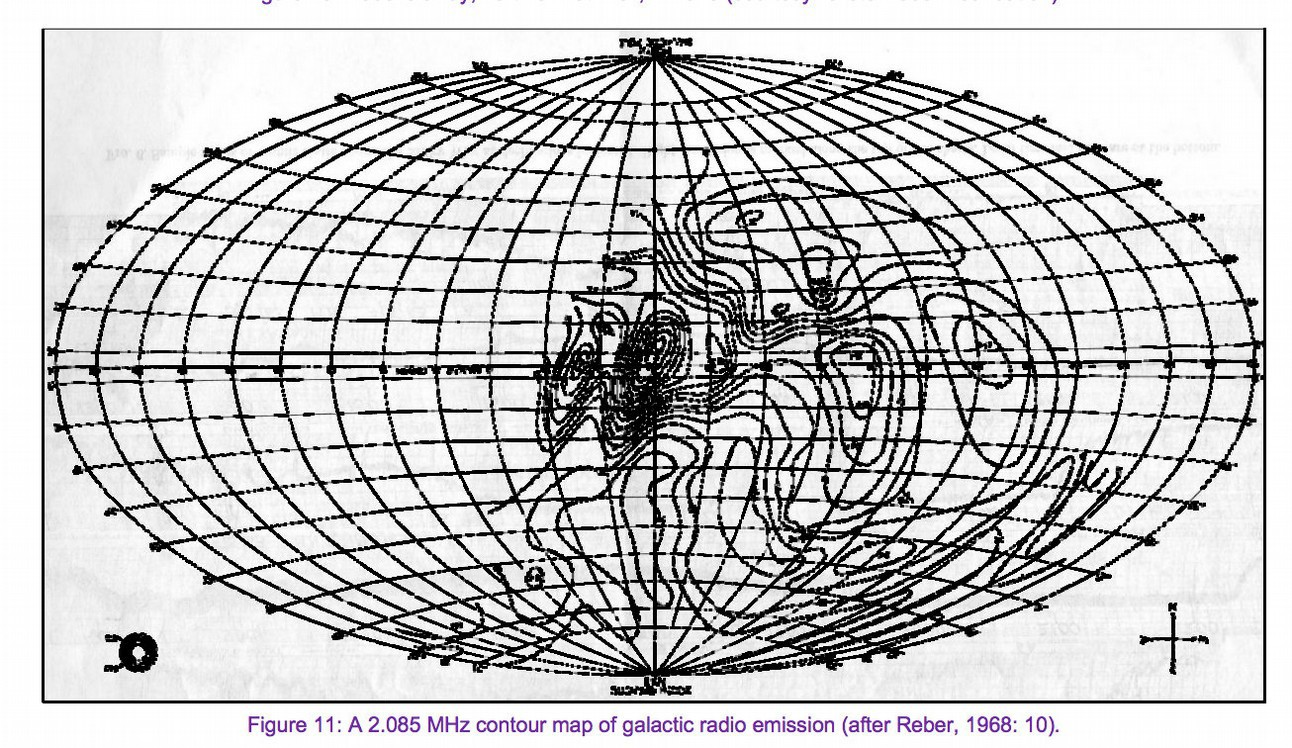
\includegraphics[width=0.7\linewidth]{Figures/Rebermap}
			\caption{}
			\label{Fig:Rebermap}
		\end{figure}
	    
	    The Radio Astronomy Explorer-2 (RAE-2) operated between 25 kHz and 13 MHz, with the main science goal of radio measurements of our Galaxy, the Sun, Earth, and all the other planets. The resolution of this experiment is $\sim$10 \degree at \SI{4.7}{\mega\hertz}~\citep{1975A&A....40..365A}. \attention{[The important point to make here is that this is basically the only data we have...there's really nothing else.]} \\
	    
	    Higher-resolutionexperiments include the OVRO-LWA, Dominion Radio Astrophysical Observatory (DRAO) 22 MHz telescope, and the DRAO \SI{10}{\mega\hertz} array. The OVRO-LWA operates at frequency ranges of \SI{36.528}{\mega\hertz} and \SI{73.152}{\mega\hertz}. At these frequencies, it has an angular resolution of \SI{15}{\arcminute}~\citep{2018AJ....156...32E}. The DRAO telescope operated at 22 MHz, and its resolution ranges between $\sim$1.1 \degree - 1.7 \degree. Its primary science goal was to measure the emission from discrete sources and observe our Galaxy's emission from its environment~\citep{1999A&AS..137....7R}. The DRAO 10 MHz array operated had a resolution of $\sim$ 2  \degree, and it was first used for discrete sources and was later used to map the large-scale structure of the background radiation~\citep{1976MNRAS.177..601C}.
	    
	    \section{Structure of this Thesis}
	    
	    
	    The outline of this thesis is as follows: In Chapter 2, 
	    Marion Island is introduced, the observing location of \prizm\ and \albatros. I will also provide a summary of my voyage to Marion. Chapter 3 will provide a brief description of the \prizm\ instrument and present a brief summary of various stages in the system. Chapter 4 will provide a full description of the \albatros\ instrument. In Chapter 5, preliminary results will be presented and conclude in the same chapter.  
 
\attention{[In this section, you should also briefly summarize your specific contributions to the projects.]}
